\documentclass{article}
\usepackage{amsmath}
\usepackage{graphicx}
\begin{document}
\title{CNN}
\date{ }
\maketitle
\section{size of feature map}
given input size,padding,filter size and stride,we can determine size of feature map:$$size\,of\,feature\,map=\lfloor\frac{inputsize+2*padding-filter\,size}{stride}+1\rfloor $$By saying size,it refers to length of every index of the matrix being considered.
\par eg.Say we have that input size is $h\times w\times c$,filter size is $f_1\times f_2\times f_3$,padding $p$ and stride $s$.Then size of feature map is $a\times b\times c$ with
\begin{align*}
	&a=\lfloor\frac{h+2p-f_1}{s}+1\rfloor\\
	&b=\lfloor\frac{w+2p-f_2}{s}+1\rfloor\\
	&c=\lfloor\frac{c+2p-f_3}{s}+1\rfloor
\end{align*}
\section{image recognition(RBG)}
Input size = height$\times$width$\times$channels(corresponding to R,B,G).It is required number of filters is equal to the number of channels and add up all the convolution output to get a feature map.Conceptual diagram reads
\begin{figure}[htbp]
	\centering
	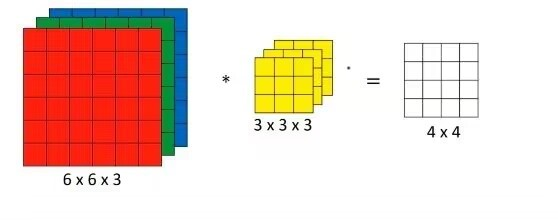
\includegraphics[width=0.5\textwidth]{1.jpg}
	\caption{RBG's filters}
\end{figure}
To actually extract more features from input,more than a set of kernels(filters) are needed.With multiple set of kernels it comes multiple set of feature maps that will eventually form a matrix with higher dimension.
\par eg.Let input size be $6\times6\times3$,kernel size be $(3\time3\time3)*2$(2 set of filters,with each possessing 3 filters sizing $3\time3$),padding be $0$ and stride be $1$.
In this example,two convolution jobs are to be done.According to the formular,one can calculate the size of each feature maps(2 in total).
\begin{align*}
	&convolution_1\rightarrow4\times4\;matrix\\
	&convolution_2\rightarrow4\times4\;matrix\\
	&gather\;two\;convolutional\;results\rightarrow4\times4\times2\;matrix
\end{align*}
\section{bias}
When feature map is finally produced,add a bias term to it elementwise with each added with the same bias.Different feature map is assigned with different biases.
\section{layer}
A convolutional layer in CNN shall include the following building blocks
\par (1) convolution between kenels and input matrix.
\par (2) biases for each feature map
\par (3) matrix of higher dimension formed by all convolutional results.
\par (4) Relu function applied to matrix in (3).
\section{number of parameters}
The number of parameters in one layer is determined its bias and kenels.A general formular that finds this number is
$$P=B+WK$$
where $P$ indicates number of parameters,$B$ represents number of different biases,$WK$ counts number of weights of all kernels.
\par eg.In one particular layer,it finds 10 filters sizing $3\times3\times3$,then the number of parameters needed in this layer is$$10+10*(3*3*3)$$
The $10$ shows in at the head of the expression is what is referred to as $B$ in the formular and the latter is $WK$.
\section{systematic process in one layer}
Let $l$ be ordinal of convoltutional layer.Elements related to layer $l^{th}$ are
\begin{align*}
	&f^{[l]}=filter\;size(In\;actuality\;,filter\;is\;mostly\;designed\;as\;square)\\
	&p^{[l]}=padding\\
	&s^{[l]}=stride\\
	&n^{[l]}_C=number\;of\;channels\\
	&N^{[l]}=number\;of\;sets\;of\;kernels\\
	&Input:n^{[l-1]}_H\times n^{[l-1]}_W\times n^{[l-1]}_C\\
	&Output:n^{[l]}_H\times n^{[l]}_W\times n^{[l]}_C\\
	&Kernel:f^{[l]}\times f^{[l]}\times n^{[l-1]}_C\\
\end{align*}
With these,output size of layer $l^{th}$ is automatically
$$n^{[l]}_k=\lfloor\frac{n^{[l-1]}+2p^{[l]}-f^{[l]}}{s^{[l]}+1}\rfloor,k=H,W$$
while channel of this layer is preset as $n^{[l]}_C$.
This can be visualized via a diagrammatic instance
\begin{figure}[htbp]
	\centering
	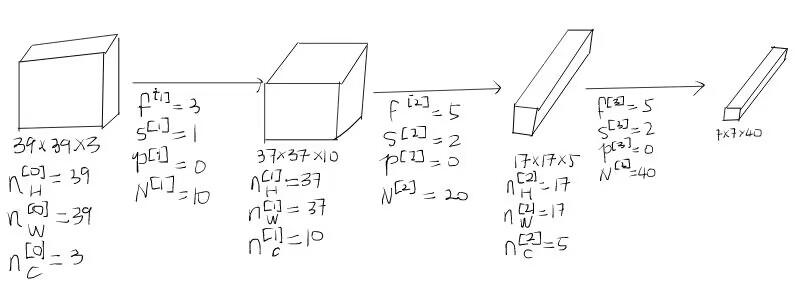
\includegraphics[width=0.8\textwidth]{2.jpg}
	\caption{visulization of systematic process}
\end{figure}
\vspace{\textheight}
\section{Pooling(max pooling)}
Max pooling is almost identical to convolution except that it uses kernnel to max-pick the element in selected window.An instant example will be the following diagram,
\begin{figure}[htbp]
	\centering
	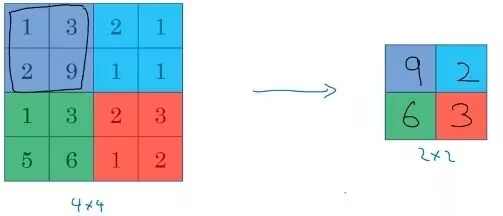
\includegraphics[width=0.6\textwidth]{3.jpg}
	\caption{max pooling}
\end{figure}
where the pooling filter sizes $4\times4$ and the first sliding window picks out 9 as it is the biggest in current window.
\par parameters of a pooling kernel should include:(1)filter sizes;(2)stride;(3)and generally no padding and they are preset so need not to learn.
\par If the pooling object is of multi-channels then it shall do max pooling channel-wise.Size of the output of pooling can be calculated the way output size of convolution is calculated.
\par eg.Let a pooling filter size $3\times3$ and input size $5\times5$,then pooling process can be explained also by a diagram:
\begin{figure}[htbp]
	\centering
	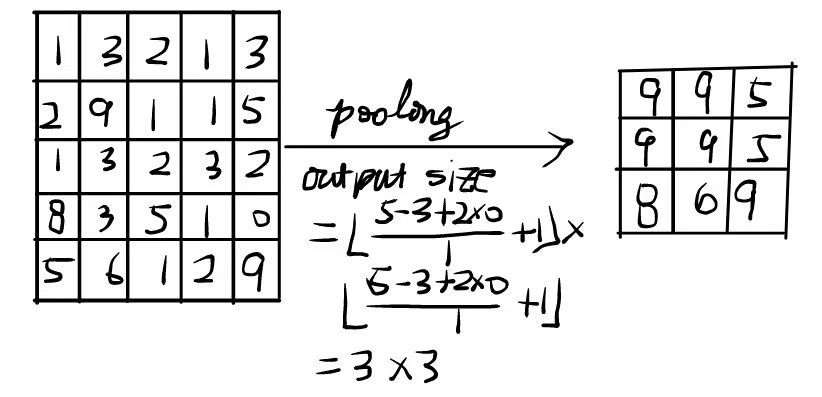
\includegraphics[width=0.6\textwidth]{4.jpg}
	\caption{pooling process}
\end{figure}
\section{Building blocks of CNN}
To construct a CNN,one must consider the following three types of layers
\par (1)Convolutional layer (CONV)
\par (2)Pooling layer (POOL)
\par (3)Fully connected layer,like softmax layer (FC)
\end{document}